% !TEX root = illustrator_submission.tex

\section{Illustrator Rendering Architecture}
\label{sec:background}

\begin{figure}[tb]
  \center{
     %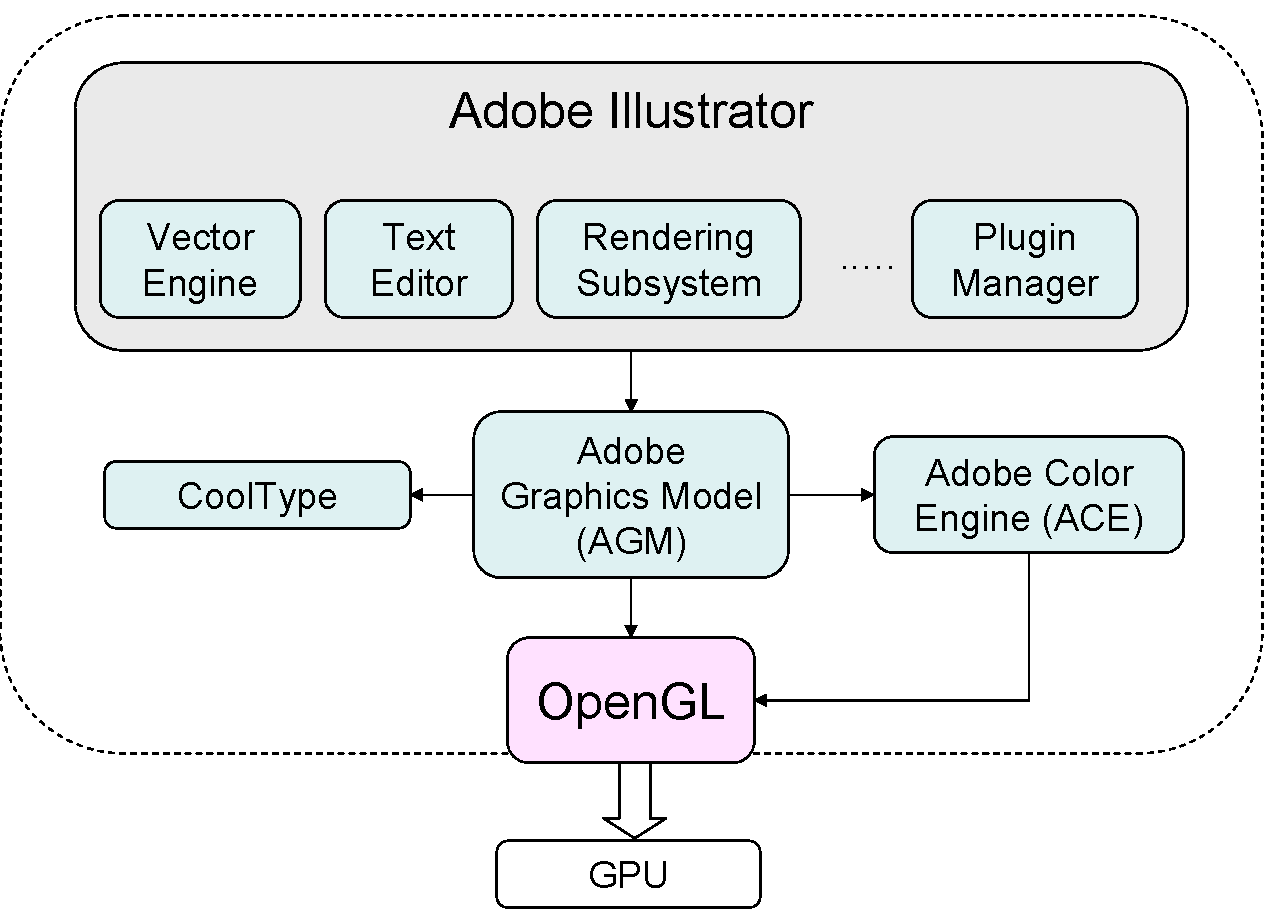
\includegraphics[width=2.6in]{images/IllustratorBlockDiagram.pdf}
     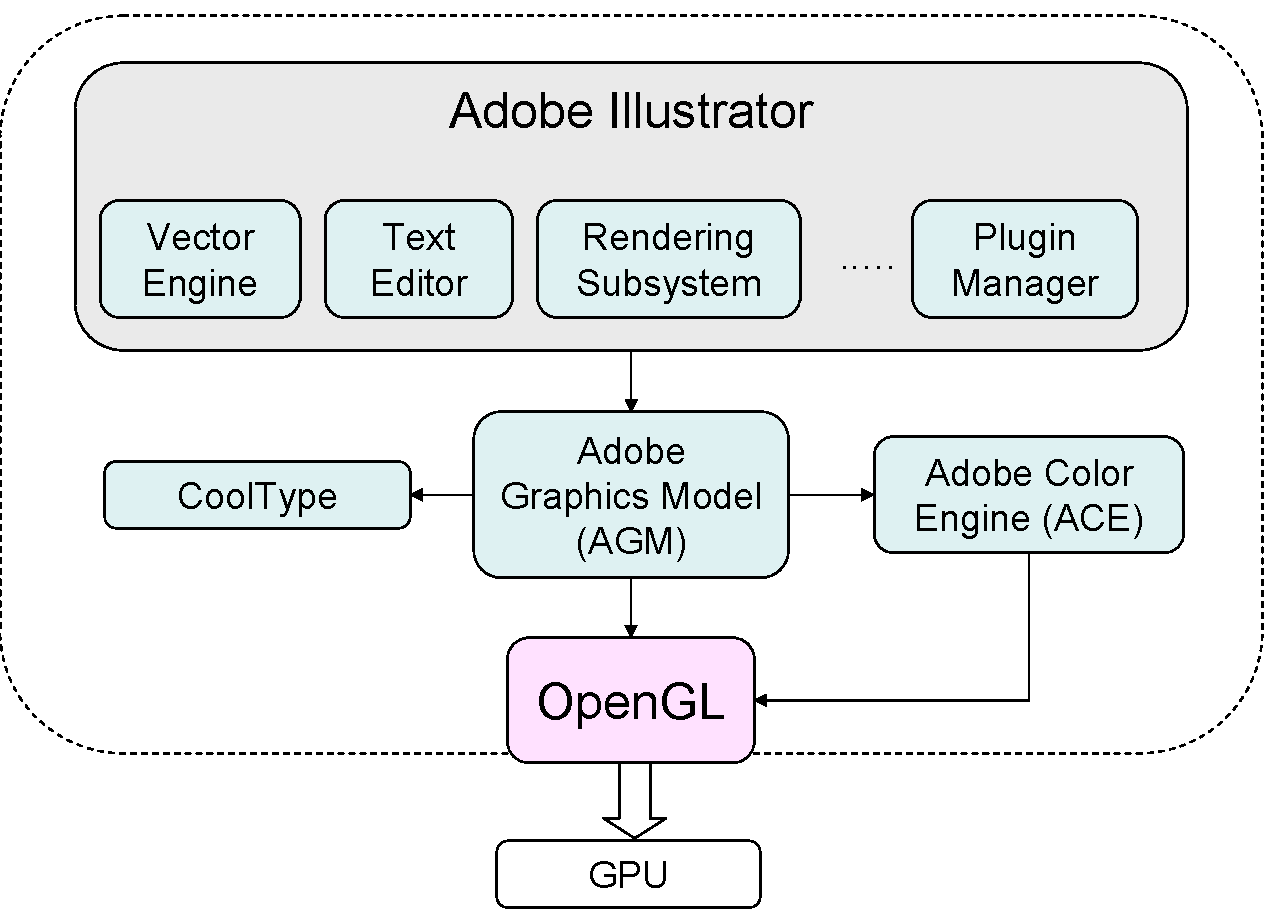
\includegraphics[width=\columnwidth]{images/IllustratorBlockDiagram.pdf}
  }
  \caption{Organization of major rendering-related modules within \Illustrator/.}
  \label{fig:illustrator-block-diagram}
\end{figure}

The software architecture of \Illustrator/ comprises several interoperable modules shown in
Figure~\ref{fig:illustrator-block-diagram} that have evolved over decades.

\ifdefined\NOSHOW
These include:
\begin{itemize}
\item
Vector Engine for creating and manipulating content with cubic B\'{e}zier splines. 
\item
Text Editor which implements rich text editing features and font handling.
\item
Plugin Manager for dynamically extending functionality (e.g. 3D support, cartography, etc.) using pluggable components (including third party plugins).
\end{itemize}
\fi

Our paper focuses on the Rendering Subsystem
for rasterizing vector content at arbitrary resolutions
so any further detail
about other modules is beyond our scope.  Despite the
complexity of \Illustrator/ overall, our GPU-acceleration effort required modifying
only the Rendering Subsystem and its subcomponents.
	
\AnIllustrator/ {\em artwork} (analogous to a 3D scene graph but for vector graphics) comprises
multiple art objects (B\'{e}zier-based path, text, image, mesh, etc.), each
attributed with a collection of {\em appearances} (fill and stroke with solid color,
pattern, gradient, etc.) and {\em effects} on these appearances (blur, feather,
shadow, etc.). When stacked in Z-order, these art objects interact with
each other to produce rich content. This interaction (or composition)
is based in the PDF specification. \Illustrator/ also provides several
high level primitives that are not supported directly in the PDF
specification but are reducible to PDF constructs. An example is an
\Illustrator/ path with both fill and stroke applied, which is reduced
to two paths---a path with stroke placed on top of a path with
fill. Figure~\ref{fig:artwork-layer} shows another example where an art
object with {\em OffsetPath} and {\em OuterGlow} effects is reduced to a group
comprising three compound paths and an image.

\begin{figure}[tb]
  \center{\includegraphics[width=3.3in]{images/artwork_layer.png}}
  \caption{How high-level artwork with effects applied (left) for a treble clef scene (center) reduces to a tree of PDF constructs (right).}
  \label{fig:artwork-layer}
\end{figure}

In service to the Rendering Subsystem, the {\em \AdobeGraphicsModel/} (\AGM/) layer
provides a pipeline for rendering PDF compliant artwork using the CPU
and now---with our work---the GPU.
For managing the color output by a target device, \AGM/ uses
\AdobeColorEngine/ (ACE) which implements color conversions
between different profiles on the GPU using GLSL shaders.
ACE profile management handles many different target devices (monitor, mobile devices, printer, etc.)
to ensure accurate color reproduction.
Font support is
implemented via \CoolType/ that provides programming interfaces for retrieving
font and glyph information (including glyph outlines) from system
fonts.
Figure~\ref{fig:illustrator-block-diagram} shows the relationship of
\AGM/, ACE, CoolType and OpenGL.
Our acceleration effort focused essentially entirely
on accelerating \AGM/ so we rely on higher level graphics primitives to be
reduced to the PDF rendering model.
